% XeLaTeX: ./build.ps1 or bash build.sh.
\documentclass[12pt,a4paper]{article}
\usepackage{fontspec,polyglossia}
\setdefaultlanguage{russian}
\setotherlanguage{english}
\setmainfont{Times New Roman}
\setmonofont{Consolas}
\usepackage{amsmath,amssymb,graphicx,booktabs,float,geometry,setspace}
\usepackage{xcolor,listings}
\usepackage[unicode,hidelinks]{hyperref}
\geometry{left=25mm,right=20mm,top=20mm,bottom=20mm}
\onehalfspacing
\setlength{\parindent}{1.25cm}
\setlength{\emergencystretch}{2em}
\graphicspath{{figures/}}
\lstset{language=Python,basicstyle=\ttfamily\small,frame=single,
  rulecolor=\color{black!20},breaklines=true,columns=fullflexible,showstringspaces=false}
% Generated by lab5.py --generate
\newcommand{\SimulationSeed}{20261101}
\newcommand{\ConstantOne}{0{,}388068}
\newcommand{\ConstantTwo}{0{,}00097825}
\newcommand{\LambdaThirty}{0{,}069834}
\newcommand{\LambdaOneTwenty}{0{,}033513}
\newcommand{\RingOneP}{0{,}2769}
\newcommand{\RingTwoP}{0{,}2000}
\newcommand{\RingOneFraction}{0{,}2543}
\newcommand{\RingTwoFraction}{0{,}2450}
\newcommand{\RingOneLong}{0{,}2714}
\newcommand{\RingTwoLong}{0{,}2114}
\newcommand{\DiffractedCount}{645}
\newcommand{\SlopeTwo}{204{,}683}
\newcommand{\InterceptTwo}{0{,}00601}
\newcommand{\RSquaredTwo}{0{,}9999998}
\newcommand{\SlopeThree}{250{,}660}
\newcommand{\InterceptThree}{0{,}00886}
\newcommand{\RSquaredThree}{0{,}9999999}


\begin{document}
\begin{titlepage}
\begin{center}
\begin{spacing}{1.3}
\textbf{МИНИСТЕРСТВО ОБРАЗОВАНИЯ РЕСПУБЛИКИ БЕЛАРУСЬ}\\[0.25cm]
\textbf{БЕЛОРУССКИЙ ГОСУДАРСТВЕННЫЙ УНИВЕРСИТЕТ}\\[0.25cm]
\textbf{ФАКУЛЬТЕТ МЕХАНИКО-МАТЕМАТИЧЕСКИЙ}\\[0.25cm]
\textbf{Кафедра веб-технологий и компьютерного моделирования}
\end{spacing}
\vspace{4.2cm}
\textbf{ВОЛНЫ ДЕ БРОЙЛЯ И ДИФРАКЦИЯ ЭЛЕКТРОНОВ}\\[0.4cm]
Лабораторная работа № 5
\end{center}
\vspace{3.6cm}
\noindent\hspace*{0.48\textwidth}\begin{minipage}{0.52\textwidth}
\begin{spacing}{1.0}
Панасика Владислава Александровича\\
обучающегося 4 курса специальности\\
«Математика и компьютерные науки»\\[0.6cm]
Научный руководитель:\\
ассистент КФОиПИ,\\
Полякова Яна Владимировна
\end{spacing}
\end{minipage}
\vfill
\begin{center}Минск, 2026\end{center}
\end{titlepage}
\setcounter{page}{2}
\tableofcontents
\clearpage

\section{Физическая модель и программа}
Цель --- исследовать статистическое формирование электронограммы,
зависимость размеров колец от напряжения и определение межплоскостных
расстояний железа. Использованы $L=757$ мм, $a=2{,}87$ \AA{} и округлённые
константы из задания: $h=6{,}63\cdot10^{-34}$ Дж$\cdot$с,
$m=0{,}911\cdot10^{-30}$ кг, $e=1{,}602\cdot10^{-19}$ Кл,
$c=2{,}998\cdot10^8$ м/с.

Для электрона с кинетической энергией $T=eV$:
\begin{equation}
 \lambda=\frac hp=
 \frac{h}{\sqrt{2meV\left(1+\frac{eV}{2mc^2}\right)}}
 =\frac{C_1}{\sqrt{V_{\mathrm{кВ}}(1+C_2V_{\mathrm{кВ}})}}\ \text{\AA},
\end{equation}
где $C_1=\ConstantOne$ \AA$\cdot$кВ$^{1/2}$,
$C_2=\ConstantTwo$ кВ$^{-1}$.
Условие Вульфа--Брэгга и геометрия экрана:
\begin{equation}
 2d\sin\theta=n\lambda,\qquad
 R=L\tan2\theta\approx\frac{nL\lambda}{d},\qquad
 d=\frac a{\sqrt{h^2+k^2+l^2}}.
\end{equation}
Угол рассеяния равен $2\theta$, а не $\theta$.

Программа регистрирует независимые точечные попадания. Центры семи колец
заданы по этим формулам, азимут равномерный, радиальное размытие
нормальное с $\sigma_r=0{,}22$ мм. Вероятности прямого пучка и семи колец:
\[
 (p_0,p_1,\ldots,p_7)=(0{,}35;0{,}18;0{,}13;0{,}10;0{,}08;0{,}065;0{,}05;0{,}045).
\]
Это учебная кинематическая модель: веса каналов выбраны явно,
абсолютные интенсивности реального железа не рассчитываются.
Результаты ниже получены по модельным координатам с базовым seed $\SimulationSeed$.

Вычислительное ядро отделено от интерфейса. Фрагмент преобразования
напряжения в радиусы:
\begin{lstlisting}
def wavelength_a(voltage_kv):
    return C1 * voltage_variable(voltage_kv)

def ring_radii_mm(voltage_kv):
    return CAMERA_MM * float(wavelength_a(voltage_kv)) * ORDERS / SPACINGS_A
\end{lstlisting}
Масштаб меняет только пределы осей; радиусы хранятся в миллиметрах.
Темп вылета управляет временем отображения, не распределением вероятностей.

\clearpage
\section{Упражнение 1. Статистический характер дифракции}
При 40, 60 и 120 кВ рассмотрены первые 10, 1000 и 10\,000
попаданий каждой серии. Оси всех изображений одинаковы; вид соответствует
увеличению $\times4$ в приложении.
\begin{figure}[H]
\centering
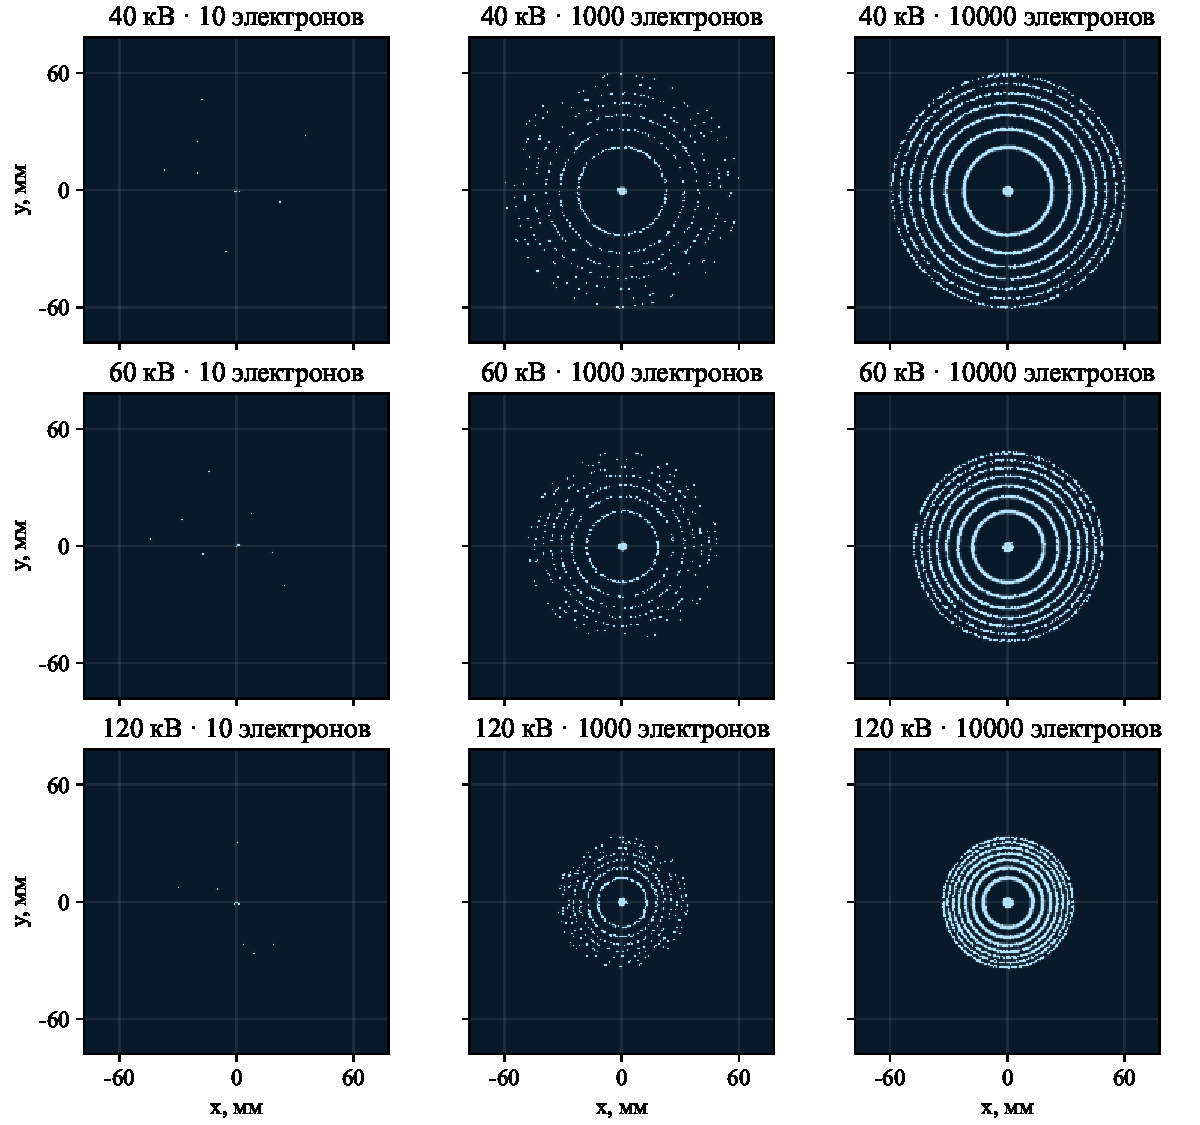
\includegraphics[width=0.96\textwidth]{task1_accumulation.pdf}
\caption{Постепенное формирование колец из отдельных попаданий.}
\end{figure}
При малом числе электронов видны отдельные точки, при большом --- кольца.
Повышение напряжения уменьшает $\lambda$ и радиусы.
Изменение темпа при фиксированном числе электронов не меняет
статистическую картину. Для одинакового seed получение 10\,000 точек
одной порцией и 100 порциями по 100 дало совпадающие координаты.

\clearpage
\subsection{Доли попаданий и закон больших чисел}
По условию $k=\sum_{j=1}^7 k_j$: прямой пучок не включён.
Для $k_0=1000$ и шага регистрации 25 исследованы два кольца:
\begin{equation}
 f_j=\frac{k_j}{k},\qquad
 q_j=\frac{p_j}{1-p_0},\qquad
 \sigma(f_j\mid k)=\sqrt{\frac{q_j(1-q_j)}{k}}.
\end{equation}
\begin{figure}[H]
\centering
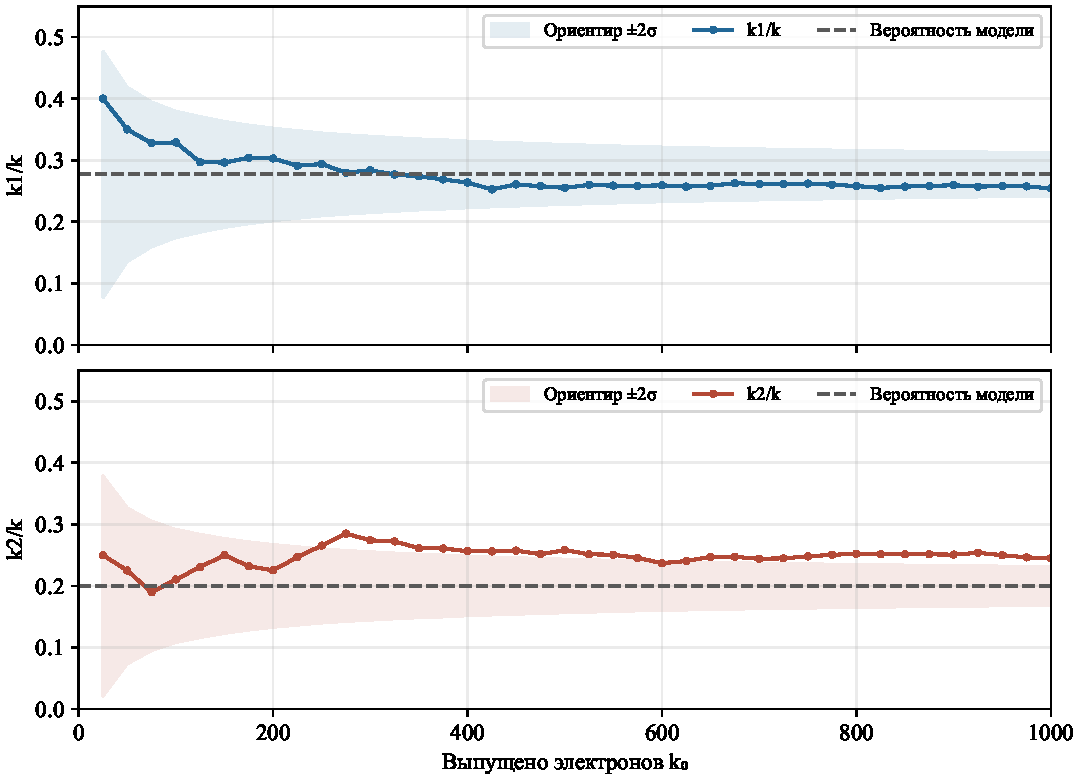
\includegraphics[width=0.91\textwidth]{task1_statistics.pdf}
\caption{Доли первого и второго колец. Затенение --- поточечный
ориентир $q_j\pm2\sigma$, не одновременный доверительный коридор траектории.}
\end{figure}
В этой серии $k=\DiffractedCount$, получены
$f_1=\RingOneFraction$, $f_2=\RingTwoFraction$ при вероятностях
$q_1=\RingOneP$, $q_2=\RingTwoP$.
При продолжении той же серии до 10\,000 электронов доли составили
$\RingOneLong$ и $\RingTwoLong$.

Частоты флуктуируют и не обязаны приближаться к вероятности монотонно.
Характерный масштаб флуктуаций уменьшается как $1/\sqrt{k}$.
Отдельные значения могут выходить за ориентир $2\sigma$;
соседние точки накопительного графика зависимы.

Физический смысл: электрон всегда регистрируется целиком в одной точке,
но распределение большого числа событий выявляет волновую закономерность.
Для образования дифракционной картины взаимодействие разных электронов
между собой не требуется.

\clearpage
\section{Упражнение 2. Зависимость радиуса от напряжения}
Для шести заданных напряжений получены серии по 20\,000 электронов.
Радиусы второго и третьего колец определены как средние расстояния
попаданий от центра внутри соответствующих кольцевых областей.
\begin{equation}
 X=\frac1{\sqrt{V(1+C_2V)}},\qquad R_j=A_jX+B_j,
 \qquad A_j^{\mathrm{теор}}=\frac{n_jLC_1}{d_j}.
\end{equation}
\begin{table}[H]
\centering
\caption{Модельные измерения; $V$ в кВ, $\lambda$ в \AA{}, $R$ в мм}
\begin{tabular}{rrrrr}
\toprule
$V$ & $\lambda$ & $X$, кВ$^{-1/2}$ & $R_2$ & $R_3$\\
\midrule
\input results/voltage_rows.tex
\bottomrule
\end{tabular}
\end{table}
\begin{figure}[H]
\centering
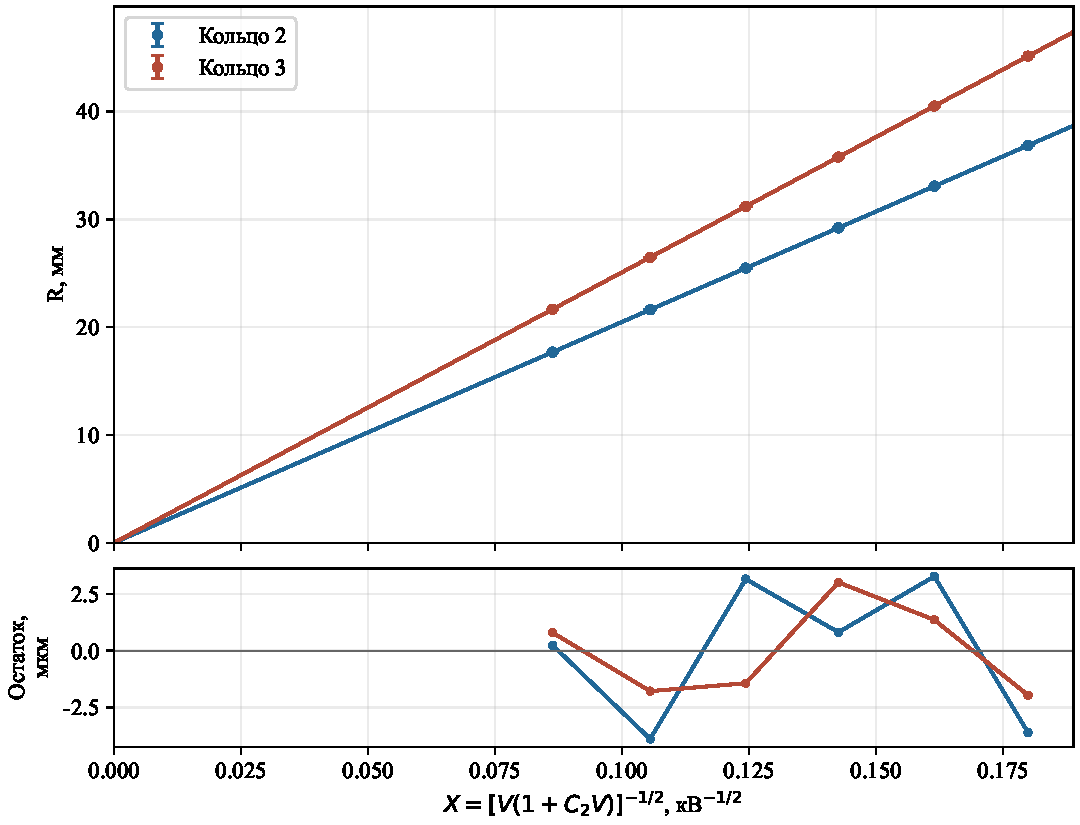
\includegraphics[width=0.79\textwidth]{task2_debroglie.pdf}
\caption{Линейная зависимость радиусов от $X$; внизу остатки аппроксимаций.}
\end{figure}
МНК дал $R_2=\SlopeTwo X+\InterceptTwo$,
$R_3=\SlopeThree X+\InterceptThree$;
$R^2=\RSquaredTwo$ и $\RSquaredThree$ соответственно.
Свободные члены близки к нулю, небольшие остатки связаны с конечной выборкой.
Полученная линейность воспроизводит соотношение де Бройля, заложенное
в модель, и не является его независимым экспериментальным доказательством.

\clearpage
\section{Упражнение 3. Межплоскостные расстояния и индексы}
Для железа при 30 кВ получена серия из 30\,000 электронов,
$\lambda=\LambdaThirty$ \AA. Средние радиусы первых пяти колец записаны
с шагом отсчёта 0,01 мм. Использованы
\begin{equation}
 d_j=\frac{n_jL\lambda}{R_j},\qquad
 S_j=\left(\frac a{d_j}\right)^2=h^2+k^2+l^2.
\end{equation}
Для кольца №4 $n=2$, для остальных $n=1$.
\begin{figure}[H]
\centering
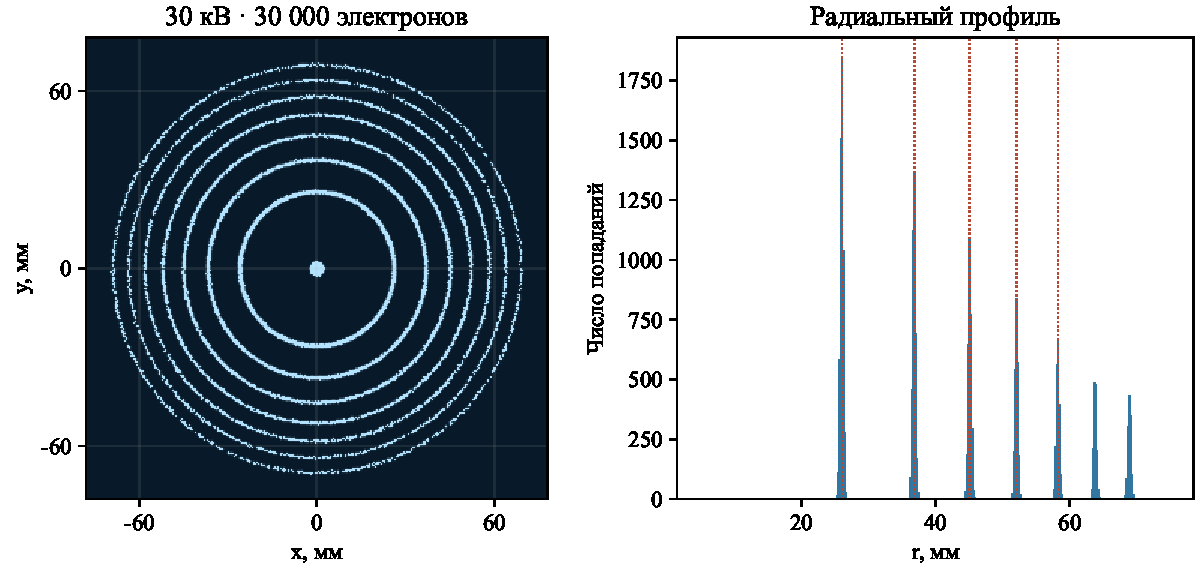
\includegraphics[width=0.84\textwidth]{task3_structure.pdf}
\caption{Электронограмма 30 кВ и радиальный профиль с первыми пятью кольцами.}
\end{figure}
\begin{table}[H]
\centering
\caption{Результаты определения структуры}
\begin{tabular}{rrrrrrr}
\toprule
№ & $n$ & $R$, мм & $d$, \AA & $S$ & $[S]$ & $(hkl)$\\
\midrule
\input results/structure_rows.tex
\bottomrule
\end{tabular}
\end{table}
Индексы найдены перебором целых $h\ge k\ge l\ge0$ после округления $S$.
Для ОЦК-структуры железа дополнительно проверено чётное $h+k+l$.
Четвёртое кольцо соответствует $(110)$ второго порядка; это та же
геометрия, что $(220)$ первого порядка, а не отдельное дополнительное кольцо.

\section*{Вывод}
Кольца формируются из одиночных попаданий и сжимаются при увеличении
напряжения. По радиусам восстановлены межплоскостные расстояния и индексы.
Такой анализ используется для определения структуры тонких образцов.
\end{document}
